\chapter{Numerical Methods}
\section{Introduction}
To discretize and evolve the system of partial differential equations, including the \gls{les} \gls{sgs} terms, we use \textit{PeleC} \cite{PeleC1, PeleC2}. \textit{PeleC} is a highly scalable code for heterogeneous architectures that is being developed as part of the \gls{ecp} through the \gls{doe}. 

For spatial discretization, \textit{PeleC} contains a few variations of the general \gls{ppm} originally derived by Colella and Woodward \cite{1984JCoPPPM}. We utilize a variation that allows for extrema preservation in the presence of steep gradients \cite{MILLER200226, COLELLA20087069}. \textit{PeleC} also has two options available time-stepping: an explicit second-order \gls{mol} formulation and an iterative scheme base on a \gls{sdc} approach \cite{SDC_PeleC}. For this work, we use the \gls{sdc} method. 

The rest of this chapter is outlined as follows: first we introduce the general finite volume formulation for conservative systems as this forms the basis of \textit{PeleC}, with an additional note on the foundations in \textit{AMReX}. The remaining sections cover the numerical methods chosen from those available in \textit{PeleC}, with motivation provided as to why they were selected for this work and a basic overview of the method. For additional details as to the specific implementations of said methods within \textit{PeleC}, please see the sources referenced throughout, in addition to the general \textit{PeleC} documentation page \cite{PeleC_doc} and Github repository \cite{PeleC_Github}; the full code is available for download and use. See Appendix \ref{Pelec-Inputs} for input parameters used in this work.  

\section{Finite Volume Formulation} \label{FVM_section}
\textit{PeleC} utilizes a finite volume formulation \cite{} to discretize the system given in Equation \eqref{filtered_NSE_FINAL}. First, we re-write a slightly modified version of this system in a condensed tensor notation, where the diffusive fluxes have been moved to the right-hand side of the original expression: 
\begin{equation} \label{NSE_tensor}
\dfrac{\partial \vb{U}}{\partial t} + \nabla \cdot \vb{F} = \nabla \cdot \vb{D}
\end{equation}
where $\vb{U}$ is the vector of conserved quantities $(\rho, \rho \vb{u}, \rho E)$, $\vb{F}$ contains the advective fluxes, and $\vb{D}$ contains the diffusive terms. Note we have dropped the filter notation from the previous section for ease and simplicity of writing but again we are working with the filtered interpretation of the compressible Navier-Stokes Equations as derived in Equation \eqref{filtered_NSE_FINAL}. 

In the finite volume formulation, the domain is sub-divided into $i$ cells, each with volume $V_i$. In \textit{PeleC}, these cells are given by boxes in Cartesian coordinates. We then integrate the system in Equation \eqref{NSE_tensor} over each finite volume to get the following:
\begin{equation} \label{FVM_app}
\int\limits_{V_i} \dfrac{\partial \vb{U}}{\partial t}\, dV + \int\limits_{V_i} \nabla \cdot \vb{F}\, dV = \int\limits_{V_i} \nabla \cdot \vb{D}\, dV
\end{equation}
In this formulation, a volume average of the state variables are considered through the following definition:
\begin{equation} \label{FVM_avg}
\vb{U}_i = \dfrac{1}{V_i} \int\limits_{V_i} \vb{U} \, dV
\end{equation} 
Applying the definition given by Equation \eqref{FVM_avg} to Equation \eqref{FVM_app} along with the divergence theorem yields the following:
\begin{equation} \label{FVM}
\dfrac{d\vb{U}_i}{dt} + \dfrac{1}{V_i} \int\limits_{S_i} \vb{F}\cdot \vb{n}\, dS = \dfrac{1}{V_i} \int\limits_{S_i} \vb{D} \cdot \vb{n} \, dS 
\end{equation}
where $S_i$ is the surface of cell $V_i$. To discretize further, the convective and diffusive fluxes must be approximated at the faces of each surface $S_i$ in order to get the total flux contributions to the system:
\begin{equation} \label{FVM_df}
\dfrac{d\vb{U}_i}{dt} +  \dfrac{1}{V_i} \sum\limits_j S_{i,j} \overbar{\vb{F}}_{i,j} =  \dfrac{1}{V_i}\sum\limits_j S_{i,j} \overbar{\vb{D}}_{i,j}
\end{equation}
where $S_{i,j}$ is the $j$-th edge of cell $i$, and corresponding subscripts on fluxes imply flux through that equivalent edge. Further methods may then be applied to perform the flux approximations needed and to discretize in time the system established in Equation \eqref{FVM_df}. 

\textit{PeleC} leverages \textit{AMReX} \cite{amrex1, amrex2, amrex3}, a block-structured hierarchical adaptive mesh refinement library for meshing infrastructure, including grid refinement, distributed parallelism, geometry representation, and output \cite{PeleC1}. Data management within \textit{AMReX} is generally structured as follows: grids are represented by Boxes. Each Box is associated with a data container known as a FAB. A MultiFAB manages a collection of FABs, which store data at each \gls{amr} level \cite{PeleC1}. Refinement ratios must be even and equally implemented in each direction. Figure \ref{amr_ex} shows an example of this type of refinement hierarchy using a refinement ratio of two for three levels of mesh refinement. Grid refinement is based on user-specified error criteria, those of which for this work are described in Chapter 4. For further details on \textit{AMReX}, see \cite{amrex1}. 

\begin{figure}[h!]
\begin{center}
	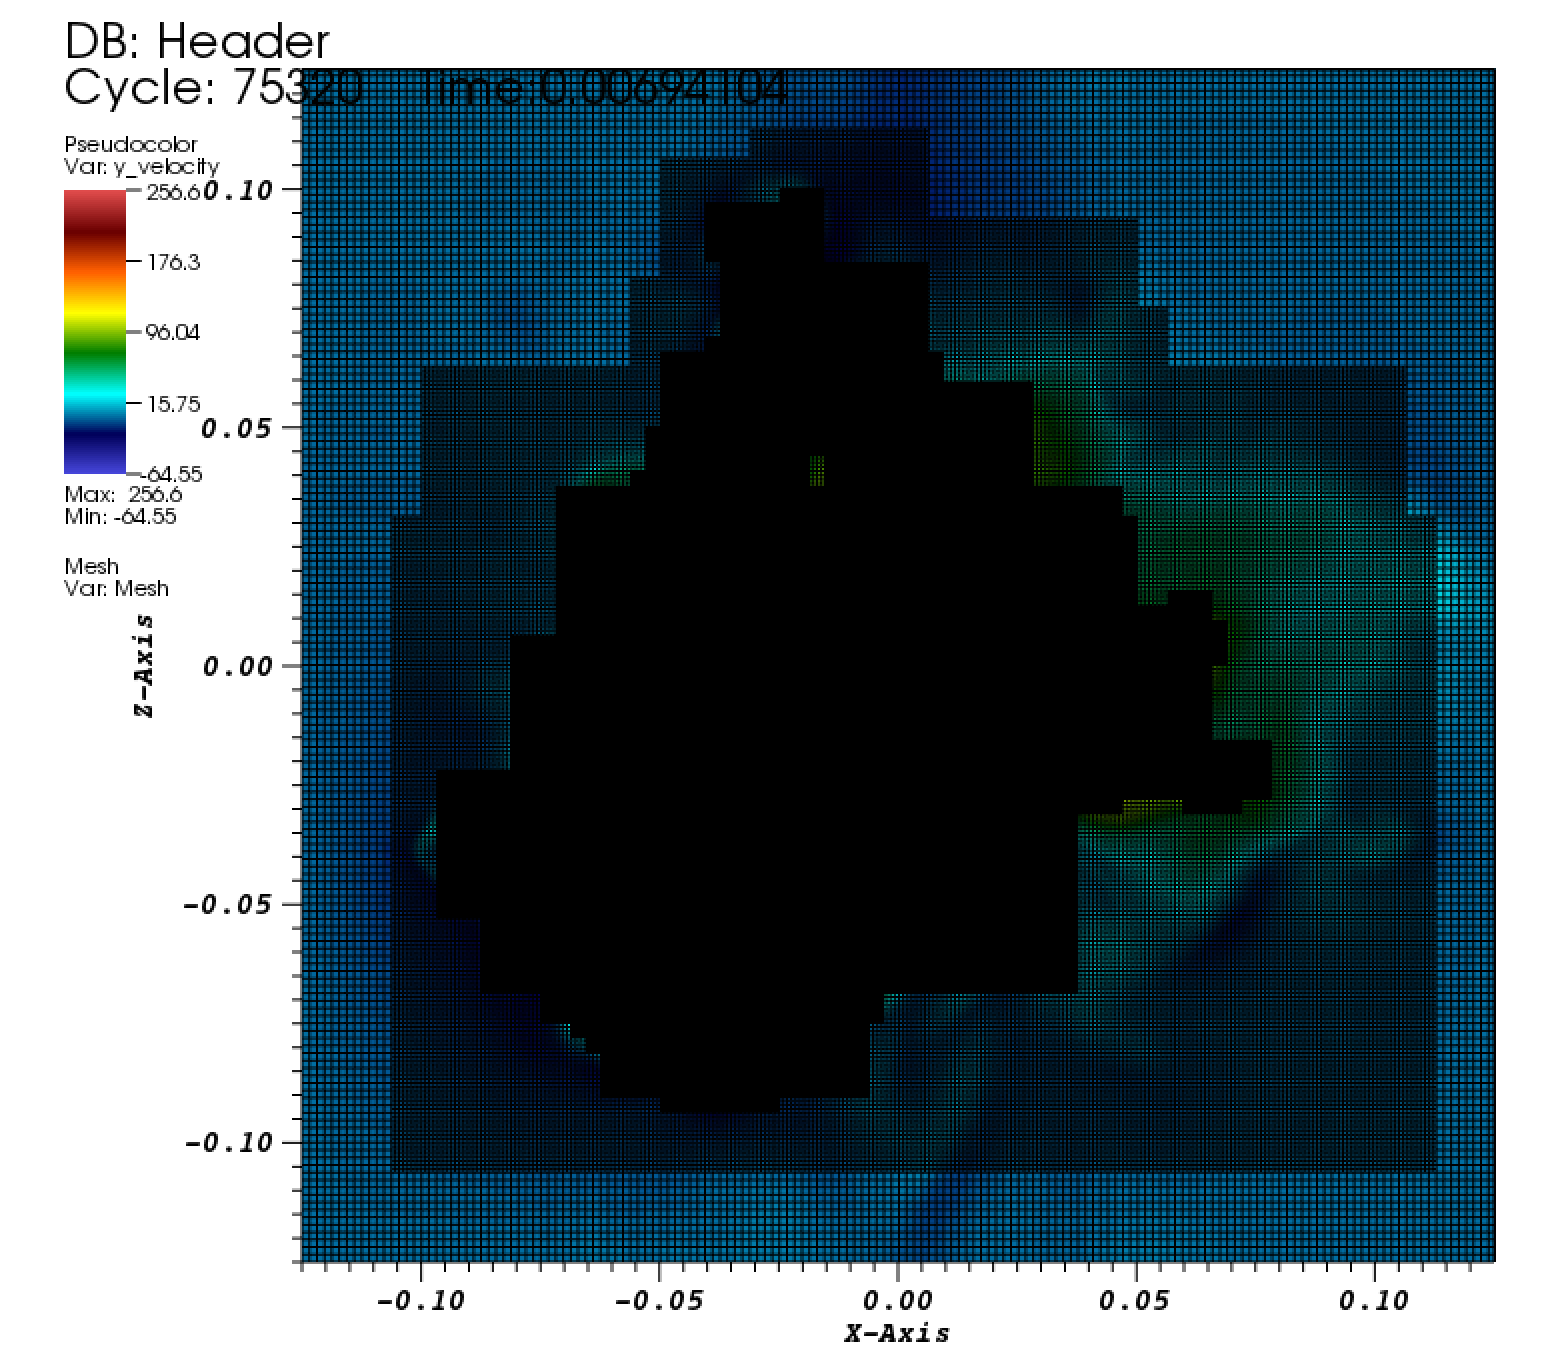
\includegraphics[scale=.3]{figures/amr_example.png}
	\caption{2D slice of 3D data demonstrating mesh refinement using \textit{AMReX}. The refinement ratio is 2 and there are 3 levels of mesh refinement.} \label{amr_ex}
\end{center}
\end{figure}

\section{Temporal Discretization: Spectral Deffered Correction Methods}
Here we present the general idea behind \gls{sdc} methods as is detailed in \cite{MISDC_general}. Consider an \gls{ode} of the following form: 
\begin{equation} \label{toy_ode}
\begin{split}
\phi_t &= F(\phi(t), t), \quad t \in [t^n, t^{n+1}], \\
\phi(t^n) &= \phi^n 
\end{split}
\end{equation}
with a solution given by the following integral expression:
\begin{equation}
\phi(t) = \phi^n + \int\limits_{t^n}^{t} F(\phi) d\tau
\end{equation}
Then, given an approximation $\phi^{(k)}(t)$ to $\phi(t)$, one can define a residual as follows:
\begin{equation} \label{sdc_residual}
E(t, \phi^{(k)}) = \phi^n + \int\limits_{t^n}^t  F(\phi^{(k)}) d\tau - \phi^{(k)}(t)
\end{equation}
Defining the error to be $\delta^{(k)}(t) = \phi(t) - \phi^{(k)}(t)$, one can then get the error as follows:
\begin{equation} \label{sdc_error}
\delta^{(k)}(t) = \int\limits_{t^n}^{t} \left[ F(\phi^{(k)} + \delta^{(k)}) - F(\phi^{(k)}) \right] d\tau + E(t, \phi^{(k)})
\end{equation}
Now, one can use a higher-order quadrature rule to approximate the integral in Equation \eqref{sdc_residual}. Along with using a lower-order discretization for the integral in Equation \eqref{sdc_error}, an iterative scheme can be constructed through which order of accuracy can be improved over subsequent iterative steps, up to the order of accuracy set by the quadrature. This iteration is defined as $\phi^{(k+1)} = \phi^{(k)} + \delta^{(k)}$, and using Equations \eqref{sdc_residual} and \eqref{sdc_error}, we can write an update as follows:
\begin{equation} \label{sdc_general}
\phi^{(k+1)}(t) = \phi^n + \int\limits_{t^n}^{t} \left[ F(\phi^{(k+1)}) - F(\phi^{(k)}) \right] d\tau + \int\limits_{t^n}^{t}F(\phi^{(k)}) d\tau
\end{equation}
where again the first integral in Equation \eqref{sdc_general} is approximated with a low-order discretization and the second integral is approximated using higher-order quadrature. \textit{AMReX} uses quadrature. 

In the \gls{misdc} formulation \cite{MISDC_general}, $F$ in Equation \eqref{toy_ode} can be broken up into individual processes: 
\begin{equation} \label{F_decomp}
F \equiv A(\phi) + D(\phi)
\end{equation}
where $A(\phi)$ and $D(\phi)$ are advection and diffusion processes, respectively. We initialize both the diffusive and advective flux \gls{cfl} conditions with a value of $0.9$ and then adapt as needed with the \gls{amr}. Note this decomposition now recovers the system formed through the finite volume formulation of Equation \eqref{FVM_df}. This decomposition in general also includes a reaction term, but since our system is a single species with no reactions it is omitted here. These individual processes can now be treated separately. Discussion of flux treatment is given in the next section. For further details on discretizing Equation \eqref{sdc_general} with \eqref{F_decomp} and applying this to a system of \gls{ode}s as in \eqref{FVM_df}, please see \cite{SDC_PeleC}. For the sake of this work, it is important to note that fluxes can be treated separately in a sort of operator splitting fashion and that accuracy can be set through quadrature choice, which for the methods used here is second-order. 


\section{Spatial Discretization: Flux Calculations}
Flux approximations are needed at cell faces, as outlined in Section \ref{FVM_section}. Following the methodology outlined in for the \gls{misdc} formulation, both advective and diffusive fluxes are centered in time for part of the iterative process \cite{MISDC_general}. To get the advective fluxes, the \gls{ppm} \cite{1984JCoPPPM} is employed to approximate state values near cell faces where they are then extrapolated to $n+\nicefrac{1}{2}$. These values are then used in an approximate Riemann solver \cite{COLELLA1985264} to calculate the advective fluxes at cell faces at $n+\nicefrac{1}{2}$. The diffusive fluxes are discretized in space using center difference formulation, with time-centering for the iterator given by the midpoint rule \cite{COLELLA20087069, MILLER200226}. Here we detail the \gls{ppm} a little further and highlight it's advantages for this work.
\subsection{Piecewise Parabolic Method}
\textit{PeleC} houses a few variations of the \gls{ppm}, including the original formulation by Colella and Woodward \cite{1984JCoPPPM}. The one used in this work is the ``extrema preserving" variation of the \gls{ppm} \cite{COLELLA20087069, MILLER200226} in order to aid in the handling of steep density gradients. Here we present the brief outline of the method in one dimension as is done in \cite{PPM_WENO} in order to illustrate the general procedure. 

First, the system in Equation \eqref{NSE_tensor} is recast in primitive form. In one dimension, this comes out be: 
\begin{equation} \label{NSE_primitive}
\dfrac{\partial \vb{Q}}{\partial t} + \vb{A} \dfrac{\partial \vb{Q}}{\partial x} = \vb{S_Q}
\end{equation}
where vector $\vb{Q}$ houses the primitive variables $(\rho, u, p, \rho e )$, $A$ is the matrix given by $\nicefrac{\partial \vb{F}}{\partial \vb{Q}}$, and $\vb{S_Q}$ is the diffusive terms recast in primitive form. Internal energy is now carried in $\vb{Q}$ to save on the number of calls made to the \gls{eos} during the Riemann solver. 
%In one dimension, $\vb{A}$ is given by: 
%\begin{equation} \label{A_1D}
%\vb{A} =
% \begin{pmatrix} 
%u & \rho & 0 & 0\\
%0 & u & \tfrac{1}{\rho} & 0\\
%0 & \rho c^2 & u & 0\\
%0 & \rho e + p & 0 & u
%\end{pmatrix}
%\end{equation}
%with eigenvalues:
%\begin{equation} \label{A_eigenvalues}
%\Lambda(\vb{A}) = \{u-c, u, u, u+c\}
%\end{equation}
%and left row and right column eigenvectors given by: 
%\begin{equation} \label{A_eigenvectors}
%\vb{l} = 
% \begin{pmatrix} 
%0 & - \tfrac{\rho}{2c} & \tfrac{1}{2c^2} & 0\\
%1 & 0 & -\tfrac{1}{c^2} & 0\\
%0 & 0 & -\tfrac{h}{c^2} & 0\\
%0 & \tfrac{\rho}{2c} & \tfrac{\rho}{2c^2} & 0
%\end{pmatrix} \quad
%\vb{r} = 
% \begin{pmatrix} 
%1 & 1 & 0 & 1\\
%-\tfrac{c}{\rho} & 0 & 0 & \tfrac{c}{\rho} \\
%c^2 & 0 & 0 & c^2\\
%h & 0 & 1 & h
%\end{pmatrix} 
%\end{equation}
%where $h$ is the enthalpy and $c$ is the sound speed. 

The first step in interpolating primitive values to cell edges is to take the average cross-cell difference as follows:
\begin{equation}
\delta q_i = \dfrac{1}{2}\left( q_{i+1} - q_{i-1} \right)
\end{equation}
Monotonicity is enforced with van Leer limiting \cite{VANLEER1979101}, with limited values denoted $\delta q_i^*$. Using these limited values, primitive variables can then be interpolated to cell edges:
\begin{equation}
q_{i+1/2} = q_i + \dfrac{1}{2} \left( q_{i+1} - q_i \right) - \dfrac{1}{6} \left( \delta q_{i+1}^* - \delta q_i^* \right)
\end{equation}
An additional constraint is imposed to ensure $q_{i+1/2}$ falls between adjacent cell averages. 

Next, edge state values $q_{L, i+1/2}$ and $q_{R, i-1/2}$ can be set from $q_{i+1/2}$ and $q_{i-1/2}$, respectively. An additional flattening limiter that utilizes local pressure in its construction is applied here as well. Monotonicity is also enforced again, this time across $q_{L, i+1/2}$, $q_i$, and $q_{R, i-1/2}$ within a single cell. 

Now, limited piecewise parabolic reconstruction can be achieved by computing average values swept out by parabolic profiles across each face, with the assumption that it moves at the speed of a characteristic wave $\lambda_k$. These averages have the following form:
\begin{equation} \label{ppm_avg}
\begin{split}
\mathcal{I}_+^{(k)}(q_i) &= \dfrac{1}{\sigma_k \Delta x} \int\limits_{((i+1/2 )-\sigma_k)\Delta x}^{(i+1/2)\Delta x} q_i^I(x) dx, \\
\mathcal{I}_-^{(k)}(q_i) &= \dfrac{1}{\sigma_k \Delta x} \int\limits^{((i-1/2 )+\sigma_k)\Delta x}_{(i-1/2)\Delta x} q_i^I(x) dx
\end{split}
\end{equation}
with $\sigma_k = |\lambda_k |\Delta t/\Delta x$, where $\lambda_k = \{u-c, u, u, u+c\}$ and $\Delta t$ and $\Delta x$ are the discretization step size in time and space, respectively. With the parabolic profile $q_i^I(x)$ given by:
\begin{equation}
\begin{split}
q_i^I(x) &= q_{R,i-1/2} + \xi(x) \left[ q_{L, i+1/2} - q_{R, i-1/2} + q_{i,6}\left( 1 - \xi(x) \right) \right] \\
q_{i,6} &= 6q_i - 3 \left( q_{R, i-1/2} + q_{L,i+1/2}\right) \\
\xi(x) &= \dfrac{x - x_{i-1/2}}{\Delta x}, \quad x_{i-1/2} \leq x \leq x_{i+1/2}
\end{split}
\end{equation}
the integrals in Equation \eqref{ppm_avg} can be explicitly written as follows:
\begin{equation}
\begin{split}
\mathcal{I}_+^{(k)}(q_i) &= q_{L, i+1/2} - \dfrac{\sigma_k}{2} \left[ q_{L,i+1/2} - q_{R,i-1/2} - \left( 1 - \dfrac{2}{3}\sigma_k \right)q_{i,6} \right], \\
\mathcal{I}_-^{(k)}(q_i) &= q_{R, i-1/2} + \dfrac{\sigma_k}{2} \left[ q_{L,i+1/2} - q_{R,i-1/2} + \left( 1 - \dfrac{2}{3}\sigma_k \right)q_{i,6} \right] 
\end{split}
\end{equation}

Finally, these averages can now be used to perform a characteristic tracing to get the time-centered left and right edge states, $q_{L, i+1/2}^{n+1/2}$ and $q_{R, i-1/2}^{n+1/2}$. Full expressions for these edge states can be found in \cite{}, along with the appropriate eigenvalue and eigenvectors needed for this procedure. With the edge states approximated, the advective fluxes can then be calculated via an approximate Riemann solver.


\subsection{Approximate Riemann Solver}
\textit{PeleC} uses the approximate Riemann solver developed by Colella and Glaz \cite{COLELLA1985264}. This Riemann solver features two iterative scheme options for calculating the classical post-discontinuity state values $\vb{u}^*$ and $p^*$: a Secant method and a Newton iteration. Full details for these implementations can be found in \cite{COLELLA1985264}. The key feature of this solver that is beneficial to this problem is the treatment of the \gls{eos} terms. Special consideration is given in formulation of this method to reduce the number of calls to the \gls{eos} within these iterative loops in order to make the method computationally tractable. This is of particular importance for cubic or higher order \gls{eos}. 


